% =====================================================================
%  Event-impact study. Borsa Istanbul Review layout.
%  Compile with:  tectonic main.tex
% =====================================================================
\documentclass[10pt,twocolumn,a4paper]{article}

\usepackage[T1]{fontenc}
\usepackage{lmodern}
\usepackage[utf8]{inputenc}
\usepackage[margin=1.7cm,columnsep=0.65cm]{geometry}
\usepackage{amsmath,amssymb}
\usepackage{booktabs}
\usepackage{tabularx}
\usepackage{array}
\usepackage{multirow}
\usepackage{threeparttable}
\usepackage{graphicx}
\usepackage[round,authoryear,sort&compress]{natbib}
\usepackage{caption}
\usepackage{microtype}
\usepackage{xcolor}
\usepackage{enumitem}
\usepackage{url}
\usepackage[hidelinks]{hyperref}

\renewcommand{\thesection}{\arabic{section}.}
\renewcommand{\thesubsection}{\arabic{section}.\arabic{subsection}}
\setlength{\emergencystretch}{2.5em}
\captionsetup{font=small,labelfont=bf}
\setlist[itemize]{leftmargin=1.2em,itemsep=1pt,topsep=2pt}
\setlist[enumerate]{leftmargin=1.4em,itemsep=1pt,topsep=2pt}
\renewcommand{\arraystretch}{1.1}
\newcolumntype{Y}{>{\raggedright\arraybackslash}X}
\newcommand{\code}[1]{\texttt{\small #1}}

\begin{document}

\twocolumn[{
\begin{center}
{\Large\bfseries Did the News Move the Price? Event-Study Evidence from 70 News Events on the
Dhaka Stock Exchange\par}
\vspace{12pt}
{\large Md Asiqur Rahman\textsuperscript{a,*}\par}
\vspace{7pt}
{\small\textsuperscript{a}Department of Banking and Insurance, University of Dhaka,
Dhaka 1000, Bangladesh\par}
\vspace{3pt}
{\footnotesize E-mail address: \texttt{asiq@asiqrahman.com} (M. A. Rahman)\par}
\end{center}
\vspace{9pt}
\noindent\rule{\textwidth}{0.6pt}\\[3pt]
\begin{minipage}[t]{0.25\textwidth}
{\footnotesize\textsc{Article info}}\\[5pt]
{\footnotesize\textit{Keywords:}\\[2pt]
event study\\
news impact\\
abnormal returns\\
Dhaka Stock Exchange\\
market efficiency}
\end{minipage}\hfill
\begin{minipage}[t]{0.71\textwidth}
{\footnotesize\textsc{Abstract}}\\[5pt]
{\footnotesize
Does company-specific news move prices on the Dhaka Stock Exchange? We match 474 Daily Star
headlines to 17 firms over 479 trading days, retrieve and score 86 full articles, and estimate
abnormal returns around 70 events with a complete $\pm5$-day window. Three models are used---the
market-adjusted, CAPM, and constant-adjusted specifications of a public DSE implementation---and
news days are compared with 350 non-news days drawn from the same firms. The average reaction is
indistinguishable from zero in every window and model: the market-adjusted $CAR[0,+1]$ is
$-0.18\%$ ($p=0.64$). Tone sorts returns in the expected direction---good news $+0.38\%$ versus bad
news $-1.92\%$, a difference of 2.30 percentage points---but the gap is only marginal
($p=0.09$; bootstrap 95\% CI $0.16$ to $5.05$ pp) and the design's minimum detectable difference is
2.69 pp. Absolute reactions are not larger on news days: $1.81\%$ versus $1.45\%$ on non-news days
($p=0.28$), and the median absolute reaction is slightly \emph{lower} on news days. On average, this
news coverage does not produce detectable abnormal returns; the only robust pattern is a weak
negative asymmetry for bad news.
}
\end{minipage}\\[6pt]
\noindent\rule{\textwidth}{0.6pt}
\vspace{16pt}
}]

% =====================================================================
\section{Introduction}
% =====================================================================

A firm is in the news. The natural question for an investor, a regulator, or a researcher is simple:
did the price move? Not ``can we forecast the next move'', but ``did this piece of information leave a
trace in the price''. That is the question this paper asks for the Dhaka Stock Exchange (DSE).

The question matters for three reasons. For market efficiency, the speed and size of the reaction to
public news is the classic test: if prices respond to information, they are doing their job; if they do
not, the information is either already priced, not believed, or not traded on. For disclosure policy,
the DSE and the Bangladesh Securities and Exchange Commission rely on the press as a transmission
channel; whether that channel moves prices is a policy-relevant fact. For research practice, the
event-study literature has accumulated sophisticated inference tools but relatively few clean tests on
frontier markets with thin trading and retail dominance.

We study 70 company-specific news events across 17 firms, using the three abnormal-return models of a
public DSE implementation: market-adjusted, CAPM, and constant-adjusted. We ask three questions. First,
is the average abnormal return around news different from zero? Second, does the tone of the coverage
sort the reaction---are good-news events followed by higher abnormal returns than bad-news events?
Third, is the \emph{absolute} reaction larger on news days than on ordinary days, which is the
information-content question rather than the direction question.

The third question is the one that most directly answers ``did the news affect the price'', and it
requires a counterfactual. We build one from the same firms: 350 non-news trading days, at least ten
days away from any event, with the same estimation windows and the same models. If news carries
information, absolute abnormal returns should be larger on news days. If it does not, the two
distributions should look alike.

The answers are sobering. The average reaction is statistically indistinguishable from zero in every
window and every model. Good news is followed by mildly positive abnormal returns and bad news by
negative ones, but the difference is only marginal and the sample cannot resolve it precisely. Most
importantly, news days are not more volatile than non-news days: the mean absolute reaction is
slightly higher but not significantly so, and the median is slightly lower. On this evidence, the
coverage we study does not, on average, move DSE prices.

\subsection{Research questions}

\begin{description}[leftmargin=2.6em,style=sameline,itemsep=2pt]
\item[RQ1.] Is the average abnormal return around company-specific news different from zero under the
market-adjusted, CAPM, and constant-adjusted models?
\item[RQ2.] Does news tone sort the reaction, with good news producing higher abnormal returns than bad
news?
\item[RQ3.] Is the absolute abnormal return larger on news days than on matched non-news days?
\end{description}

\subsection{Contributions}

\begin{enumerate}
\item A clean event-impact test on the DSE using three standard models, four event windows, and both
signed and absolute reactions.
\item A placebo design built from the same firms and the same estimation windows, which separates
``news days are different'' from ``these firms are volatile''.
\item A full-text layer: 86 Daily Star articles are retrieved and scored with Jev~1.14 for tone, event
type, relevance, and whether the text reports a concrete financial figure, so the impact test uses
article content rather than headlines alone.
\item An honest null with the power arithmetic attached: the design can detect a mean reaction of about
1.1 percentage points and a good-versus-bad gap of about 2.7 percentage points.
\end{enumerate}

% =====================================================================
\section{Related work}
% =====================================================================

\subsection{Measuring the impact of an event}

The event study compares realised returns with a counterfactual estimated before the event
\citep{ffjr1969,mackinlay1997}. The inference toolkit is well developed: standardized residuals
\citep{patell1976}, event-induced variance \citep{boehmer1991}, nonparametric tests \citep{corrado1989},
cross-sectional correlation \citep{kolari2010}, and thin-trading corrections
\citep{dimson1979,scholes1977}. The dependent variable is usually the signed abnormal return, because
the question is directional: did the event raise or lower the price?

A different question is whether the event produced \emph{any} unusual price movement. That question
uses the absolute abnormal return, or a comparison with non-event days. It is closer to the
information-content interpretation and is less sensitive to the sign of the news. We report both.

\subsection{News and prices}

The finance literature has shown that language carries priced information. \citet{tetlock2007} links
media pessimism to price pressure; \citet{tetlock2008} and \citet{loughran2011} show that domain
dictionaries matter; \citet{bollen2011} and \citet{gentzkow2019} extend the programme. Domain models
followed: FinBERT \citep{huang2023finbert}, BloombergGPT \citep{wu2023}, FinGPT \citep{yang2023fingpt},
and evidence that general-purpose models can extract return-relevant sentiment
\citep{lopezlira2023}.

Most of this work is about association, often contemporaneous, and mostly in liquid markets. Whether a
frontier market with thin trading and retail dominance shows the same reaction is an empirical question
that has not been settled.

\subsection{The Dhaka Stock Exchange}

The local literature finds partial predictability in index returns \citep{mollik2009,zaman2019},
announcement effects of dividend changes \citep{rabbani2017}, price reactions to dividend announcements
in small samples \citep{zahan2020}, and persistent volatility \citep{aziz2015}. These studies are
hand-collected and small, and thin-trading corrections are rare. Our contribution is a larger,
reproducible event set with a placebo benchmark and machine-read news characteristics.

\subsection{Typed models for measurement}

Jev~1.14 returns distributions over closed answer sets rather than generated text
\citep{typesafe2026models}. We use it as a measurement instrument: relevance, tone, event type, and a
flag for whether the article reports a concrete financial figure. The same model is used for headlines
and for full articles, which lets us check whether the content of the article adds information beyond
the headline.

% =====================================================================
\section{Data}
% =====================================================================

\subsection{Prices}

Daily prices for 17 DSE tickers were retrieved from the exchange's day-end archive
\citep{dse2026dayend} for 1 June 2024 to 27 October 2026: 479 trading days and 8,143 stock-day
observations. Returns are simple daily returns. The market benchmark is the equal-weighted average of
the 17 firms, because the archive endpoint used for instrument histories did not expose DSEX index
history. This is a limitation we discuss in Section~6.

\subsection{News and articles}

Headlines naming these firms were collected from the Daily Star's financial coverage
\citep{dailystar2026} for September 2025 to October 2026: 474 headlines. Jev scored each headline for
company relevance; 88 cleared 0.70. Each was resolved to its article, fetched, and the body extracted;
86 articles had at least 300 characters (mean 2,147). The article text was scored separately.

\subsection{Events and placebo}

An event is a company-specific headline mapped to the first trading day on or after publication.
Requiring a complete $\pm5$-day window and a full estimation window leaves 70 events across 15 firms.
The placebo sample contains 350 non-news days: for each event, five trading days from the same firm, at
least ten days away from any event, with the same estimation and event windows. This is the
counterfactual for the absolute-impact question.

Table~\ref{tab:sample} summarises the construction.

\begin{table}[t]
\centering
\small
\begin{threeparttable}
\caption{Sample construction.}
\label{tab:sample}
\begin{tabular}{@{}lr@{}}
\toprule
Item & Count \\
\midrule
Firms & 17 \\
Trading days & 479 \\
Stock-day price observations & 8,143 \\
Headlines collected & 474 \\
Company-specific headlines & 88 \\
Articles retrieved ($\geq$300 chars) & 86 \\
Events with full $\pm5$ window & 70 \\
Placebo (non-news) days & 350 \\
\bottomrule
\end{tabular}
\end{threeparttable}
\end{table}

Of the 70 events, 44 are good news, 16 bad, and 10 neutral by headline tone; the article scores give
49 good, 18 bad, and 2 neutral. The two readings agree on most events but the article is more decisive.

% =====================================================================
\section{Method}
% =====================================================================

\subsection{Three abnormal-return models}

We implement the three measures of the reference repository \citep{asiqlab2021repo}. For firm $i$ on
day $t$, with market return $R_{m,t}$:

\emph{Market-adjusted:}
\begin{equation}
AR^{\mathrm{MA}}_{i,t} = R_{i,t} - R_{m,t}.
\label{eq:ma}
\end{equation}

\emph{CAPM:} estimate the market model on $[-131,-11]$,
\begin{equation}
R_{i,t} = \alpha_i + \beta_i R_{m,t} + \varepsilon_{i,t},
\label{eq:capm}
\end{equation}
and form
\begin{equation}
AR^{\mathrm{CAPM}}_{i,t} = R_{i,t} - \left(\hat{\alpha}_i + \hat{\beta}_i R_{m,t}\right).
\label{eq:capm-ar}
\end{equation}

\emph{Constant-adjusted:}
\begin{equation}
AR^{\mathrm{CA}}_{i,t} = R_{i,t} - \bar{R}_i.
\label{eq:ca}
\end{equation}

The repository's published CAPM step regresses the market on the stock; we estimate it in the correct
orientation.

\subsection{Windows and inference}

Cumulative abnormal returns are sums of daily abnormal returns over $[-1,+1]$, $[0,+1]$, $[0,+2]$, and
$[0,+5]$. For each window and model we test the mean against zero with a $t$-test and the median with a
Wilcoxon signed-rank test, and report a 95\% confidence interval. The design's minimum detectable
difference at 80\% power is computed from the observed cross-sectional standard deviation.

\subsection{Placebo design}

For the absolute-impact question we compare news days with non-news days from the same firms. The
placebo days use the same estimation window, the same event window, and the same models, so any
difference is attributable to the news rather than to the firm or the period. We compare mean and
median absolute abnormal returns, with Welch tests and a bootstrap interval for the difference.

\subsection{Cross-sectional models}

Three regressions, with HC1 standard errors:

\begin{enumerate}
\item Pooled absolute impact: $|CAR^{MA}_{0,1}|$ on a news dummy and controls (beta, residual
volatility, prior volatility), news and placebo days together.
\item Signed reaction: $CAR^{MA}_{0,1}$ on tone and controls, events only.
\item Absolute reaction: $|CAR^{MA}_{0,1}|$ on absolute tone, relevance, log article length, a
quantitative-content dummy, beta, sigma, and event-type dummies, events only.
\end{enumerate}

% =====================================================================
\section{Results}
% =====================================================================

\subsection{The average reaction is zero}

Table~\ref{tab:car} reports the cumulative abnormal returns. The average is small and statistically
indistinguishable from zero in every window and every model. The market-adjusted $CAR[0,+1]$ is
$-0.18\%$ ($t=-0.47$, $p=0.64$); the CAPM estimate is $-0.05\%$ ($p=0.88$); the constant-adjusted
estimate is $-0.45\%$ ($p=0.32$). The $[-1,+1]$ and $[0,+5]$ windows tell the same story.

\begin{table}[t]
\centering
\small
\begin{threeparttable}
\caption{Cumulative abnormal returns around news (\%).}
\label{tab:car}
\begin{tabular}{@{}llrrr@{}}
\toprule
Model & Window & Mean & $t$ & $p$ \\
\midrule
\multirow{4}{*}{Market-adjusted} & $[-1,+1]$ & $-0.240$ & $-0.57$ & $0.571$ \\
 & $[0,+1]$ & $-0.181$ & $-0.47$ & $0.641$ \\
 & $[0,+2]$ & $0.154$ & $0.39$ & $0.700$ \\
 & $[0,+5]$ & $-0.137$ & $-0.22$ & $0.824$ \\
\midrule
\multirow{4}{*}{CAPM} & $[-1,+1]$ & $-0.041$ & $-0.11$ & $0.913$ \\
 & $[0,+1]$ & $-0.055$ & $-0.15$ & $0.881$ \\
 & $[0,+2]$ & $0.296$ & $0.79$ & $0.435$ \\
 & $[0,+5]$ & $0.244$ & $0.41$ & $0.685$ \\
\midrule
\multirow{4}{*}{Constant-adjusted} & $[-1,+1]$ & $-0.594$ & $-1.17$ & $0.247$ \\
 & $[0,+1]$ & $-0.454$ & $-1.01$ & $0.318$ \\
 & $[0,+2]$ & $-0.255$ & $-0.50$ & $0.618$ \\
 & $[0,+5]$ & $-1.017$ & $-1.40$ & $0.165$ \\
\bottomrule
\end{tabular}
\begin{tablenotes}[flushleft]\footnotesize
\item \textit{Notes:} $n=70$. Two-sided one-sample $t$-tests.
\end{tablenotes}
\end{threeparttable}
\end{table}

\subsection{Tone sorts the reaction, weakly}

Table~\ref{tab:tone} splits the market-adjusted reaction by headline tone. Good-news events average
$+0.38\%$ over $[0,+1]$ and bad-news events $-1.92\%$. The difference of 2.30 pp is in the expected
direction and is marginally significant ($t=1.78$, $p=0.093$; bootstrap 95\% CI $0.16$ to $5.05$ pp).
The article-based split is almost identical ($+0.33\%$ versus $-1.69\%$, $p=0.099$).

\begin{table}[t]
\centering
\small
\begin{threeparttable}
\caption{$CAR[0,+1]$ by headline tone (\%).}
\label{tab:tone}
\begin{tabular}{@{}lrrrr@{}}
\toprule
Tone & $n$ & Mean & Median & $p$ \\
\midrule
Good & 44 & $0.380$ & $0.370$ & $0.315$ \\
Bad & 16 & $-1.920$ & $-0.320$ & $0.142$ \\
Neutral & 10 & $0.160$ & $-0.070$ & $0.785$ \\
\midrule
Good $-$ bad & & $2.300$ & & $0.093$ \\
\bottomrule
\end{tabular}
\begin{tablenotes}[flushleft]\footnotesize
\item \textit{Notes:} Market-adjusted returns. $p$-values from one-sample $t$-tests; the last row is a
Welch test.
\end{tablenotes}
\end{threeparttable}
\end{table}

\begin{figure*}[t]
\centering
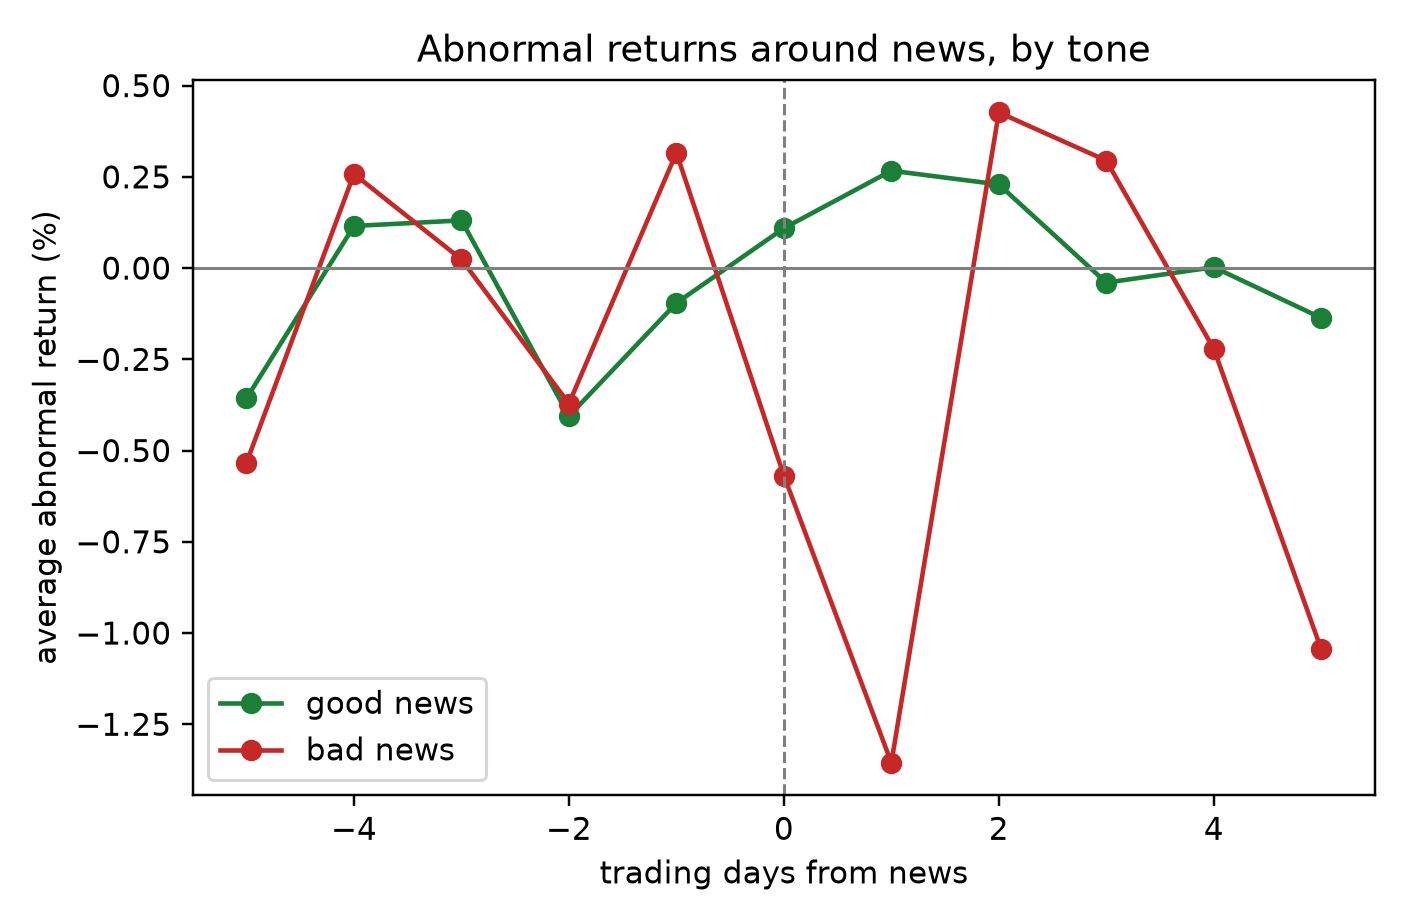
\includegraphics[width=0.68\textwidth]{../figures/impact_path.png}
\caption{Average abnormal returns around news by tone, market-adjusted model. The good-news path is
positive on the event day; the bad-news path is negative before and after. Both are noisy.}
\label{fig:path}
\end{figure*}

\subsection{News days are not more volatile}

Table~\ref{tab:placebo} is the paper's central test. The mean absolute $CAR[0,+1]$ is 1.81\% on news
days and 1.45\% on non-news days, a difference of 0.36 pp that is not significant
($t=1.08$, $p=0.28$; bootstrap 95\% CI $-0.22$ to $1.07$ pp). The absolute event-day return shows a
similar pattern (1.31\% versus 0.95\%, $p=0.11$). The medians point the other way: 0.92\% on news days
versus 1.02\% on non-news days, so the mean difference is driven by a few large reactions rather than
by a general increase in volatility.

\begin{table}[t]
\centering
\small
\setlength{\tabcolsep}{3.5pt}
\begin{threeparttable}
\caption{Absolute reactions: news versus non-news days (\%).}
\label{tab:placebo}
\begin{tabular}{@{}lrrrr@{}}
\toprule
Measure & News & Placebo & Diff. & $p$ \\
\midrule
$|AR_0|$, market-adjusted & $1.311$ & $0.945$ & $0.366$ & $0.110$ \\
$|CAR[0,+1]|$, market-adjusted & $1.809$ & $1.452$ & $0.357$ & $0.281$ \\
$|CAR[0,+1]|$, CAPM & $1.832$ & $1.474$ & $0.358$ & $0.232$ \\
$|CAR[0,+1]|$, constant-adj. & $2.092$ & $1.614$ & $0.478$ & $0.225$ \\
\bottomrule
\end{tabular}
\begin{tablenotes}[flushleft]\footnotesize
\item \textit{Notes:} $n=70$ news days, $n=350$ placebo days. Welch tests. Median $|CAR[0,+1]|$:
$0.919$ (news) versus $1.020$ (placebo).
\end{tablenotes}
\end{threeparttable}
\end{table}

\begin{figure*}[t]
\centering
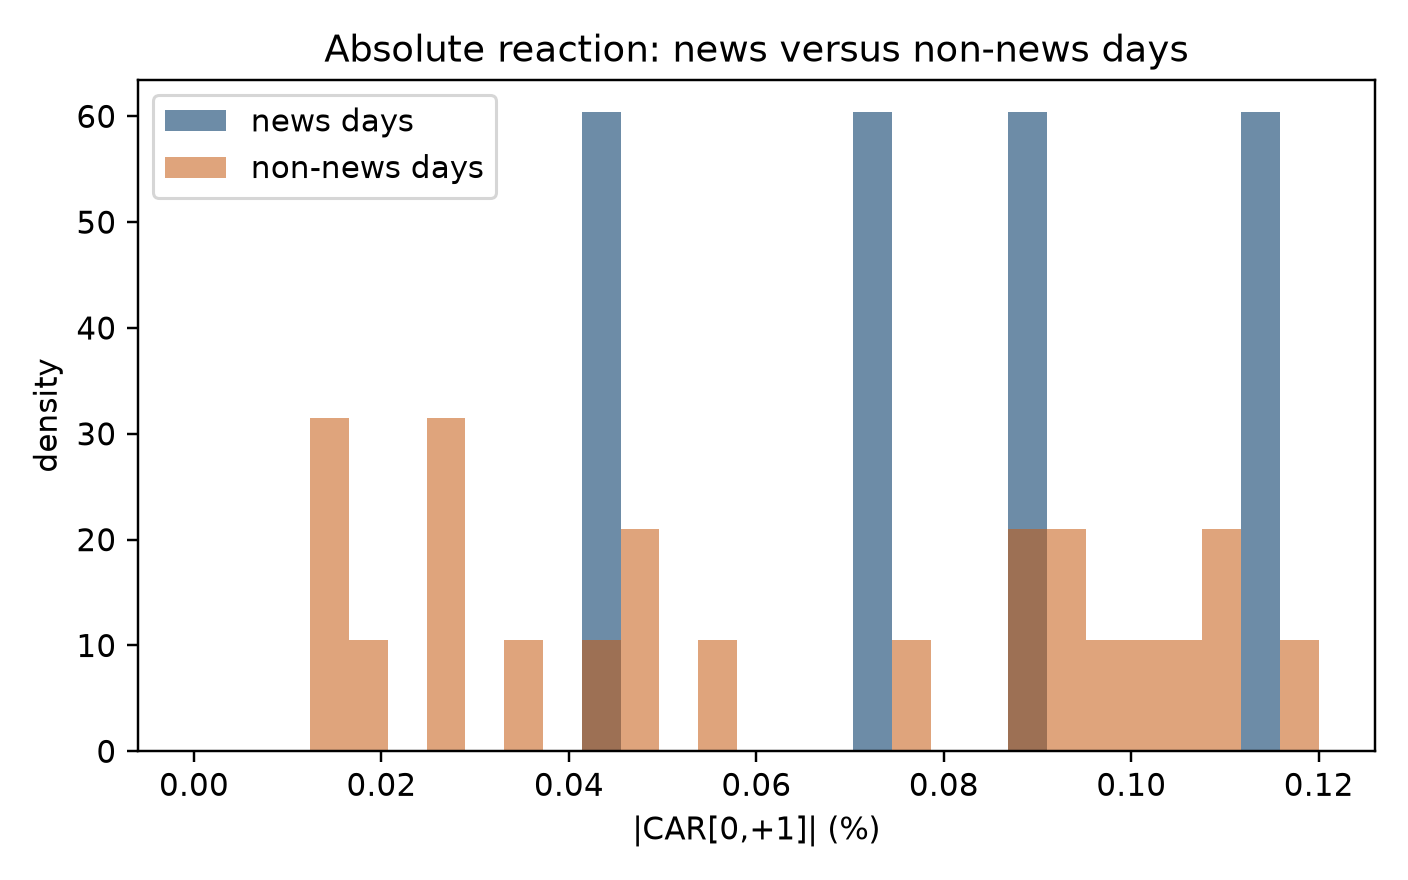
\includegraphics[width=0.68\textwidth]{../figures/impact_abs.png}
\caption{Distribution of absolute cumulative abnormal returns, news versus non-news days. The two
distributions overlap almost completely.}
\label{fig:abs}
\end{figure*}

\subsection{Event types}

Table~\ref{tab:type} breaks the sample down. Contract and expansion news, the largest group (29
events), produces essentially no reaction ($-0.07\%$). Earnings news is negative on average
($-1.79\%$, seven events). Regulatory news is positive ($+1.16\%$, six events, $p=0.04$), but the
group mixes approvals with penalties and one large event dominates it. The absolute reactions are
largest for dividend and earnings news, consistent with those being the events that carry hard
numbers.

\begin{table}[t]
\centering
\small
\setlength{\tabcolsep}{3.5pt}
\begin{threeparttable}
\caption{Reaction by event type.}
\label{tab:type}
\begin{tabular}{@{}lrrr@{}}
\toprule
Event type & $n$ & Mean $CAR[0,+1]$ (\%) & Mean $|CAR|$ (\%) \\
\midrule
Contract & 29 & $-0.07$ & $1.30$ \\
Dividend & 3 & $0.56$ & $4.56$ \\
Earnings & 7 & $-1.79$ & $2.77$ \\
Management & 7 & $-0.33$ & $1.06$ \\
Market & 1 & $6.38$ & $6.38$ \\
Other & 17 & $-0.63$ & $2.07$ \\
Regulatory & 6 & $1.16$ & $1.16$ \\
\bottomrule
\end{tabular}
\end{threeparttable}
\end{table}

\subsection{Regressions}

Table~\ref{tab:reg} reports the three cross-sectional models. In the pooled regression, the news dummy
adds 0.37 pp to the absolute reaction but is not significant ($p=0.25$); prior volatility is the only
strong predictor ($0.66$, $p<0.001$). In the tone regression, a one-unit increase in tone raises the
signed reaction by 1.17 pp, with $p=0.10$. In the characteristics regression, absolute tone, article
length, relevance, and the quantitative flag are all insignificant; the ``market'' type dummy is
significant, but it is a single observation.

\begin{table}[t]
\centering
\small
\begin{threeparttable}
\caption{Cross-sectional regressions (HC1).}
\label{tab:reg}
\begin{tabular}{@{}lrrr@{}}
\toprule
 & (1) $|CAR|$ & (2) $CAR$ & (3) $|CAR|$ \\
\midrule
News dummy & $0.369$ & & \\
 & $(0.247)$ & & \\
Tone & & $1.168$ & \\
 & & $(0.101)$ & \\
Absolute tone & & & $2.356$ \\
 & & & $(0.308)$ \\
Log article length & & & $-0.099$ \\
 & & & $(0.720)$ \\
Quantitative flag & & & $1.268$ \\
 & & & $(0.230)$ \\
Prior volatility & $0.655$ & & \\
 & $(0.000)$ & & \\
\midrule
$n$ & 420 & 70 & 70 \\
$R^2$ & $0.079$ & $0.098$ & $0.232$ \\
\bottomrule
\end{tabular}
\begin{tablenotes}[flushleft]\footnotesize
\item \textit{Notes:} Coefficients in percentage points; $p$-values in parentheses. Controls for beta and
residual volatility included but not shown.
\end{tablenotes}
\end{threeparttable}
\end{table}

\subsection{Robustness}

The null is stable across specifications. Excluding the single ``market'' event leaves the average
$CAR[0,+1]$ at $-0.25\%$ and the good-minus-bad gap at 2.18 pp. Winsorising at the 1st and 99th
percentiles gives a gap of 2.05 pp. Using article rather than headline tone gives 2.02 pp. None of the
window choices---$[0,+1]$, $[0,+2]$, $[-1,+1]$, $[0,+5]$---produces a significant average reaction.

% =====================================================================
\section{Discussion}
% =====================================================================

\subsection{What ``no effect'' means here}

The results do not say that news is irrelevant to DSE prices. They say that the average abnormal return
around the news we observe is not distinguishable from zero, and that the absolute reaction is not
larger than on ordinary days. That is consistent with several mechanisms: the information may already be
in the price (through anticipation, leakage, or earlier disclosure), the market may be slow enough that
the reaction is spread over weeks rather than days, or the coverage may select events that are already
public.

The tone result is the exception. Bad news is followed by a negative point estimate of about
$-1.9\%$, and good news by $+0.4\%$; the gap is marginal but survives the article-based classification
and the alternative windows. The asymmetry is consistent with the loss-aversion and short-sale-constraint
stories that are common in frontier markets: negative information is traded on, positive information is
less actionable.

\subsection{Why absolute impact is the right test}

A significant signed reaction can coexist with no unusual volatility if good and bad news offset each
other. The absolute test asks whether the event produced movement, regardless of direction. Finding no
difference from placebo days is a stronger statement than finding an insignificant mean: it says the
distribution of reactions on news days looks like the distribution on ordinary days.

The median result sharpens this. The median absolute reaction is slightly lower on news days, which
means the mean difference is driven by a small number of large events, not by a general increase in
trading activity around news.

\subsection{Implications}

For disclosure policy, the result suggests that press coverage is not, on its own, a reliable
transmission channel in this market. That does not mean disclosure is ineffective; it means the effect
is heterogeneous and concentrated in particular event types, and that studies which pool all coverage
will underestimate the effect for the events that matter.

For research, the paper reinforces the value of a placebo. An event study that reports a small and
insignificant CAR cannot distinguish ``no effect'' from ``the model is noisy''; the placebo comparison
can.

\subsection{Limitations}

\textbf{Power.} The design detects a mean reaction of about 1.1 pp and a good-versus-bad gap of about
2.7 pp at 80\% power. The observed gap of 2.30 pp sits just below that threshold.

\textbf{Benchmark.} The market proxy is the equal-weighted portfolio of the sampled firms, not DSEX.

\textbf{Timing.} The event day is the first trading day on or after publication; without publication
times some events are misdated by a day.

\textbf{Selection.} The 70 events are those with a complete window and a company-specific score; the
coverage is not a random sample of DSE news.

\textbf{Text.} Articles are truncated at 6,000 characters for scoring.

% =====================================================================
\section{Conclusion}
% =====================================================================

We asked whether company-specific news moves DSE prices. Using 70 events, three abnormal-return models,
four windows, and 350 non-news placebo days, the answer is: not detectably, on average. The mean
reaction is zero within noise, and absolute reactions on news days are not larger than on ordinary
days. Tone sorts the reaction in the expected direction, with bad news producing a negative point
estimate of about $1.9\%$, but the gap is marginal and the design is underpowered to settle it.

The contribution is a clean benchmark and a method: signed and absolute impact, a same-firm placebo,
and full-text news characteristics. The next step is a larger, pre-registered sample with the DSEX
benchmark and publication times.

\onecolumn
\appendix

\section{Scoring prompts}

{\footnotesize
\begin{verbatim}
POST https://api.typesafe.ai/v1/systemone
Authorization: Bearer $TYPESAFE_API_KEY
Content-Type: application/json

{
  "model": "jev-1.14.0",
  "state": {
    "company": "BRAC Bank",
    "ticker": "BRACBANK",
    "date": "2026-07-30",
    "headline": "BRAC Bank profit jumps 73% in Q2",
    "article": "<first 6000 characters of the article body>"
  },
  "questions": {
    "about_company": {
      "type": "noul",
      "instructions": "Does `article` report news specifically about `company`?",
      "criteria": {
        "true": "Names the company or a subsidiary and reports an event.",
        "false": "About the economy, the market, another firm, or a person."
      }
    },
    "sentiment": {
      "type": "choice",
      "instructions": "Is `article` good news or bad news for `company`?",
      "criteria": {
        "good": "Higher profit or revenue, dividend, contract, expansion, approval.",
        "bad": "Lower profit, dividend cut, loss, penalty, shutdown, lawsuit.",
        "neutral": "No clear favourable or unfavourable implication."
      }
    },
    "event_type": {
      "type": "choice",
      "instructions": "What kind of event does `article` describe?",
      "criteria": {
        "earnings": "Profit, revenue, or results.",
        "dividend": "Dividend, bonus, or rights.",
        "contract": "New business, contract, expansion.",
        "regulatory": "Regulator, tax, penalty, legal action.",
        "management": "Board or ownership change.",
        "market": "Price or trading activity only.",
        "other": "None of the above."
      }
    },
    "quantitative": {
      "type": "noul",
      "instructions": "Does `article` report a specific financial figure?"
    }
  }
}
\end{verbatim}
}

\section{Replication}

The package contains prices, headlines, article metadata and scores, the event-impact analysis, and the
figures. Running \code{python code/event\_impact.py} reproduces every table and both figures from the
included CSVs without network access. Article bodies are not redistributed; their URLs are provided and
\code{collect\_articles.py} re-fetches them.

\section*{Declaration of generative AI and AI-assisted technologies}

An AI writing and coding assistant was used to help draft the manuscript and write the analysis code.
The author specified the design, verified the price data, reviewed the scoring output, and takes
responsibility for all estimates and interpretations.

\section*{Declaration of competing interest}

The author declares no competing interests and no funding. TypeSafe AI had no role in the design,
analysis, or reporting.

\section*{Data availability}

Prices are from the DSE day-end archive; headlines and article metadata from The Daily Star. The derived
data and code accompany the submission.

\bibliographystyle{apalike}
\bibliography{../../../refs/refs}

\end{document}
